\section{Design of thread model}
%这一部分,我们首先分析Phoenix较差scalability的根本原因,然后针对Phoenix scalability存在的challenge,我们提出可行的解决方案,即构造一种具有较好scalability的thread model。具体的实验部分将在section6做详细的解释
{\color{red}In this section, we will search the main factor of Phoenix's bad scalability.
Then we present a new thread model, which has good scalability.
}

\subsection{Scalability of Phoenix}
In Phoenix, programs are often written to start as many threads as the system has cores,
As indicated by figure\ref{fig:phoenix:speedup}, 
when the system is larger than their scalability limit 
adding more threads might actually scale negatively.
The time of completing a workload for one core increases 
when there are more cores in the system. 
The trend of this curve suggests that
the parallel scalability of Phoenix is poor.

In order to understand the scalability behavior, 
Perf\cite{} is exploited to collect execution time information
on the function basis. 
Figure\ref{fig:phoenix:spinlock} shows the percent of \_\_ticket\_spin\_lock of each benchmark.
Histgram on 16cores and 32 cores
show that \_\_ticket\_spin\_lock is one function 
which have largest execution time with 71.25\% and 40.15\% respectively. 
Experimental results show that Phoenix suffer from serious lock contention
when the core count exceeds 8.
\bluet{From Seciton2.2, Phoenix takes two strategies to avoid lock contention.
Why the benchmarks suffer from serious lock contention?
It caused by linux kernel.}
\begin{figure}[!h!t]  
    \centering
    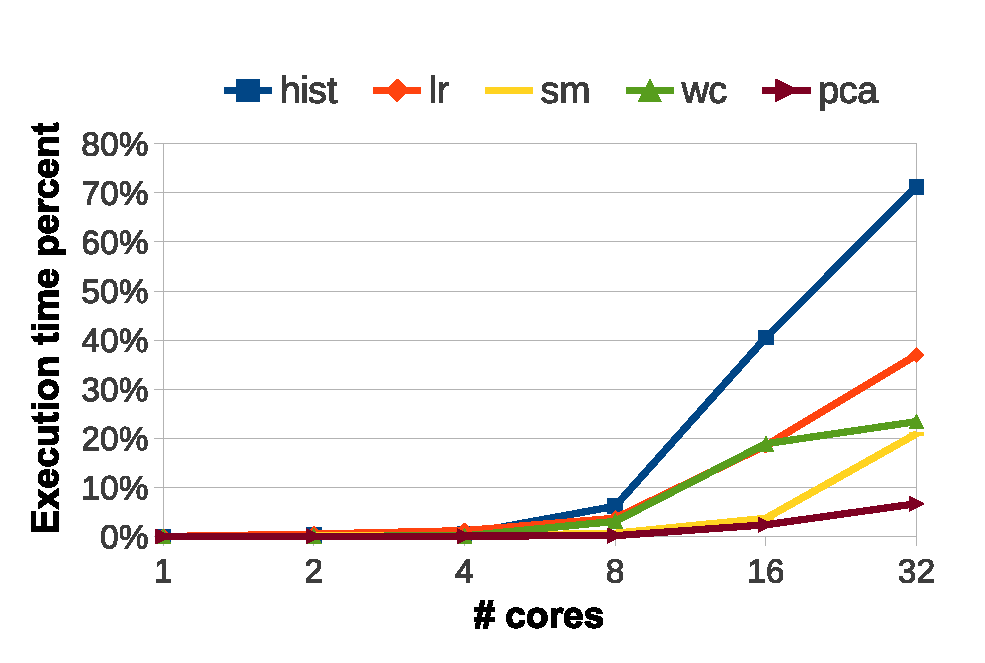
\includegraphics[width=0.35\textwidth]{eps/phoenix_spinlock.eps}
    \caption{Phoenix spinlock percent}
    \label{fig:phoenix:spinlock}
\end{figure}


%Phoenix采取了划分和barrier的方式,以避免多个线程对共享区域的的竞争,为什么还会存在如此高的spinlock呢,
There is a sense in the community that traditional kernel
designs won’t scale well on multicore processors: that
applications will spend an increasing fraction of their time
in the kernel as the number of cores increases.
To understand the Linux scalability
behavior, we analyze the related implementation of Linux
kernel and exploit performance tools to identify scalability
bottlenecks.

Data structure private locks can be a problem 
if the data structure is shared by multiple threads. 
A standard example here are the mm\_sem read-write semaphore 
that protects the list of mappings in a process and 
the pagetable\_lock that protects the pagetable state of a process. 
These locks are local to a process’ address space. 
\bluet{In Phoenix, there is one master process,
and map worker or reduce worker are threads belong to the master process}. 
However when the process is using multiple threads 
then these threads will be able to access the address space in parallel,
which can cause contention on these locks.
%Call-graph information
%and source code analysis show that the two functions are
%called when adding a virtual memory address range into the
%process address space or deleting a virtual memory address range. 
Call-graph information and source code analysis show that 
\_\_ticket\_spin\_lock is caused by pagefault.
When a large multi-threaded computing job 
that causes a lot of parallel page-faults, 
these page-faults will all run into contention on the mm\_sem semaphores.
Semaphores are sleeping locks 
and may run into convoying problems 
where waiting threads may 
get stuck at the end of the wait queue for a long time.\cite{Andi2009lmulticore}
Thus, spin lock 
contention degrades the parallel scalability performance of 
the benchmark. 


%Unfortunately these programs are often written to start as many threads as the system has CPUs, 
%but when the system is larger than their scalability limit adding more threads might actually scale negatively.
%The first measure is to limit them to the maximum number of threads that they can successfully scale to.
%This of course leaves some of the CPUs idle. 

%Performance data reveal that two functions vma link() and
%unlink file vma() have the largest execution time (46.02%
%and 49.97\%) and lock contention. Call-graph information
%and source code analysis show that the two functions are
%called when adding a virtual memory address range into the
%process address space or deleting a virtual memory address range. 
%When multiple slave processes call mmap() or unmap() concurrently, the 
%memory mapped file address range should be added into or 
%deleted from each slave process address space. However, 
%the same spin lock protecting the memory mapped file 
%address range should be held or released. Thus, spin lock 
%contention degrades the parallel scalability performance of 
%the benchmark. 



%The difference between processes and threads under Linux 2.4 is that threads share more parts of their state (address space, file handles etc) than processes, 

\subsection{Separate Address Space}
%这一部分,我们不提生产消费模型,
%为什么要进行地址空间隔离,通过新的线程模型,我们实现了地址空间隔离,隔离之后有什么好处?相比Phoenix,我们这种新的模型会不会带来开销。
One reason that widely used operating systems 
use a lock on the address space is 
that they use complex index data structures to guarantee O(log n)
lookup time when a process has many mapped memory
regions. Linux uses a red-black tree for the regions\cite{linux}. 
Because the data structures require rebalancing 
when a memory region is inserted, 
they protect the entire data structure with a single lock.
The lock is local to a process address space.
when the process is using multiple threads 
then these threads will be able to access
the address space in parallel, 
which can cause contention on the lock.
%随着核数的增多,这种问题会更加突出,最好导致较差的scalability
\bluet{As the increasing of cores number, 
the scalability will be bad.
}

We aim at providing an race-free programming abstraction 
to support scalable MapReduce.
%We aim at providing an easy-to-use programming abstraction 
%to support scalable MapReduce.
\bluet{
With this target, we propose a new thread programming model \myth(Scalable thread).
%We propose a new thread programming model to support efficient pipeline parallelism.
%新的线程模型与传统的Pthread模型的主要不同在于:(1)每个线程拥有自己独立的地址空间,这样可以避免多个线程对mm\_struct结构的竞争。(2)线程之间有一个共享的通道,同于线程数据的共享。
\myth is C library-based and 
thread in \myth run in separate memory spaces.
Threads in Pthreads share the address space of the process that created it, 
while threads in \myth have their own address space,
meaning each thread has a mm\_struct.
Therefore, thread no need contend with others thread for lock.
On the other hand,
Threads based on share space can directly communicate with other threads of its process; 
While \myth must use interprocess communication to communicate with the other threads.
We provoide a share channel for threads to communicate.
The initial state of isolated memory in a thread is inherited from
its parent thread when it is started. 
Currently, there is no shared heap among threads, 
but private heap for each thread.
On the other hand, comparing to thread, it is bad for sharing data between threads.
To solute the problem, \myth provide interface of channnel to 
create, send, receive opration.
}
\label{sec:pm:thread}
\begin{figure}[htpb]
\input chanapi.tex
\caption{Main functions of \myds thread API.}
\label{fig:api:thread}
\end{figure}



%mapreduce中是如何使用这个简易的模型进行编程和实现的,这个模型潜在的开销是什么
Figure\ref{fig:api:thread} lists main function of managing threads and channels in \myth.
Initialize in \myds, the master threads invoke 
\codet{thread\_alloc} to create map workers and reduce workers
, and invoke \codet{chan\_alloc} to alloc channels for them.
Map worker as a sender to send message(calling \codet{chan\_setprod}),
and reduce worker as a receiver to receive message(calling \codet{chan\_recv}).
After creating channels and setting up send-receive relationship,
both map and reduce workers start work by invoking \codet{thread\_start}.
When the local buffer is full, 
Map worker invoke \codet{chan\_send} to send
the key-value to coresponded channel.
Then Reduce worker invoke \codet{chan\_recv} to receive
the key-value from the channel. 
Though, using \myth can effectively decrease the overhead of contention,
it also take some extra overhead comparing to Phoneix. 
The extra overhead focus on initialization(section 5). 






\subsection{Design of the Channel}
%channel的底层实现,以及它无限制的映射机制,想说明的问题是:不需要等待,且没有过多的malloc和free操作带来的开销。
Once the channel relationships are set up, 
map workers can invoke \codet{chan\_send} to send messages to channel,
and reduce workers can receive from the channel by \codet{chan\_recv}.
%MPI中的channel是不是要等待,是不是预先分配一块固定的大小。
In order to avoid map waiting when the channel buffer is full,
we design an unbounded size of communication buffer.
Therefore, a sender can send any number of messages without blocking or waiting.
Unboundedness goal is the key to achieve high throughput.
%这个特性的好处

In order to reach a unbounded buffer,
We design an extend machanism 
which allows remap channel’s buffer to a new page frames.
To record the produce-consume dependence and 
trace generations of page frames among the sharing parties, 
a special anchor extension page is introduced and shared between producer and consumers.
Initially a sequence of pages in channel buffer 
are mapped to a \codet{anchor} page table (Anchor in Figure
\ref{fig:spmckern:extend}), 
in which each page has a corresponding page table entry (PTE).
Upon a producer page fault, the fault handler will allocate a real page frame and update the faulting page with a
writable producer mapping so that the producer can write the
page afterwards.When a consumer attempts to read a page
with invalid mapping, the fault handler will check whether
the target page frame is present and further fixed or not:
 
When a thread want to send without waiting, 
it can call extend primitive to remap channel buffer to new page frames,
without changing the old page 
that consumers may still require. 
After a consumer receive the old page from the channel, 
it can call extend to find the new page frames sended by the
producer.
The older page frames decrease their reference counts and
are freed automatically when the counts reach zero


\begin{figure}[!h!t]  
    \centering
    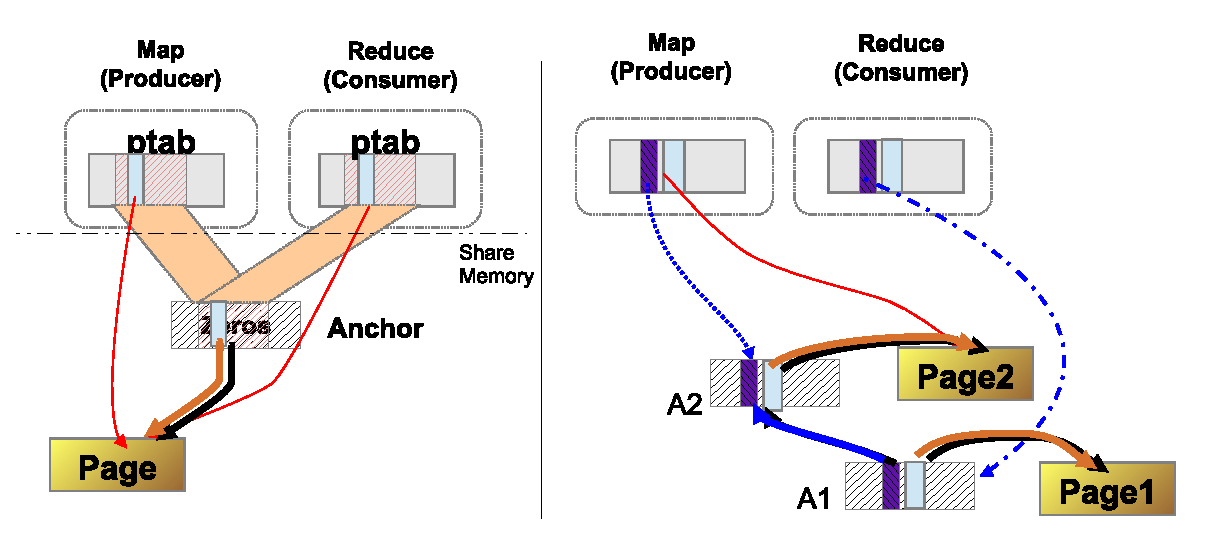
\includegraphics[width=0.5\textwidth]{eps/spmckern_extend.eps}
    \caption{channel extend machanism}
    \label{fig:spmckern:extend}
\end{figure}


%\begin{figure*}
%\centering
% \subfigure[]{
%  \label{fig:spmc:kernext:a}  
%  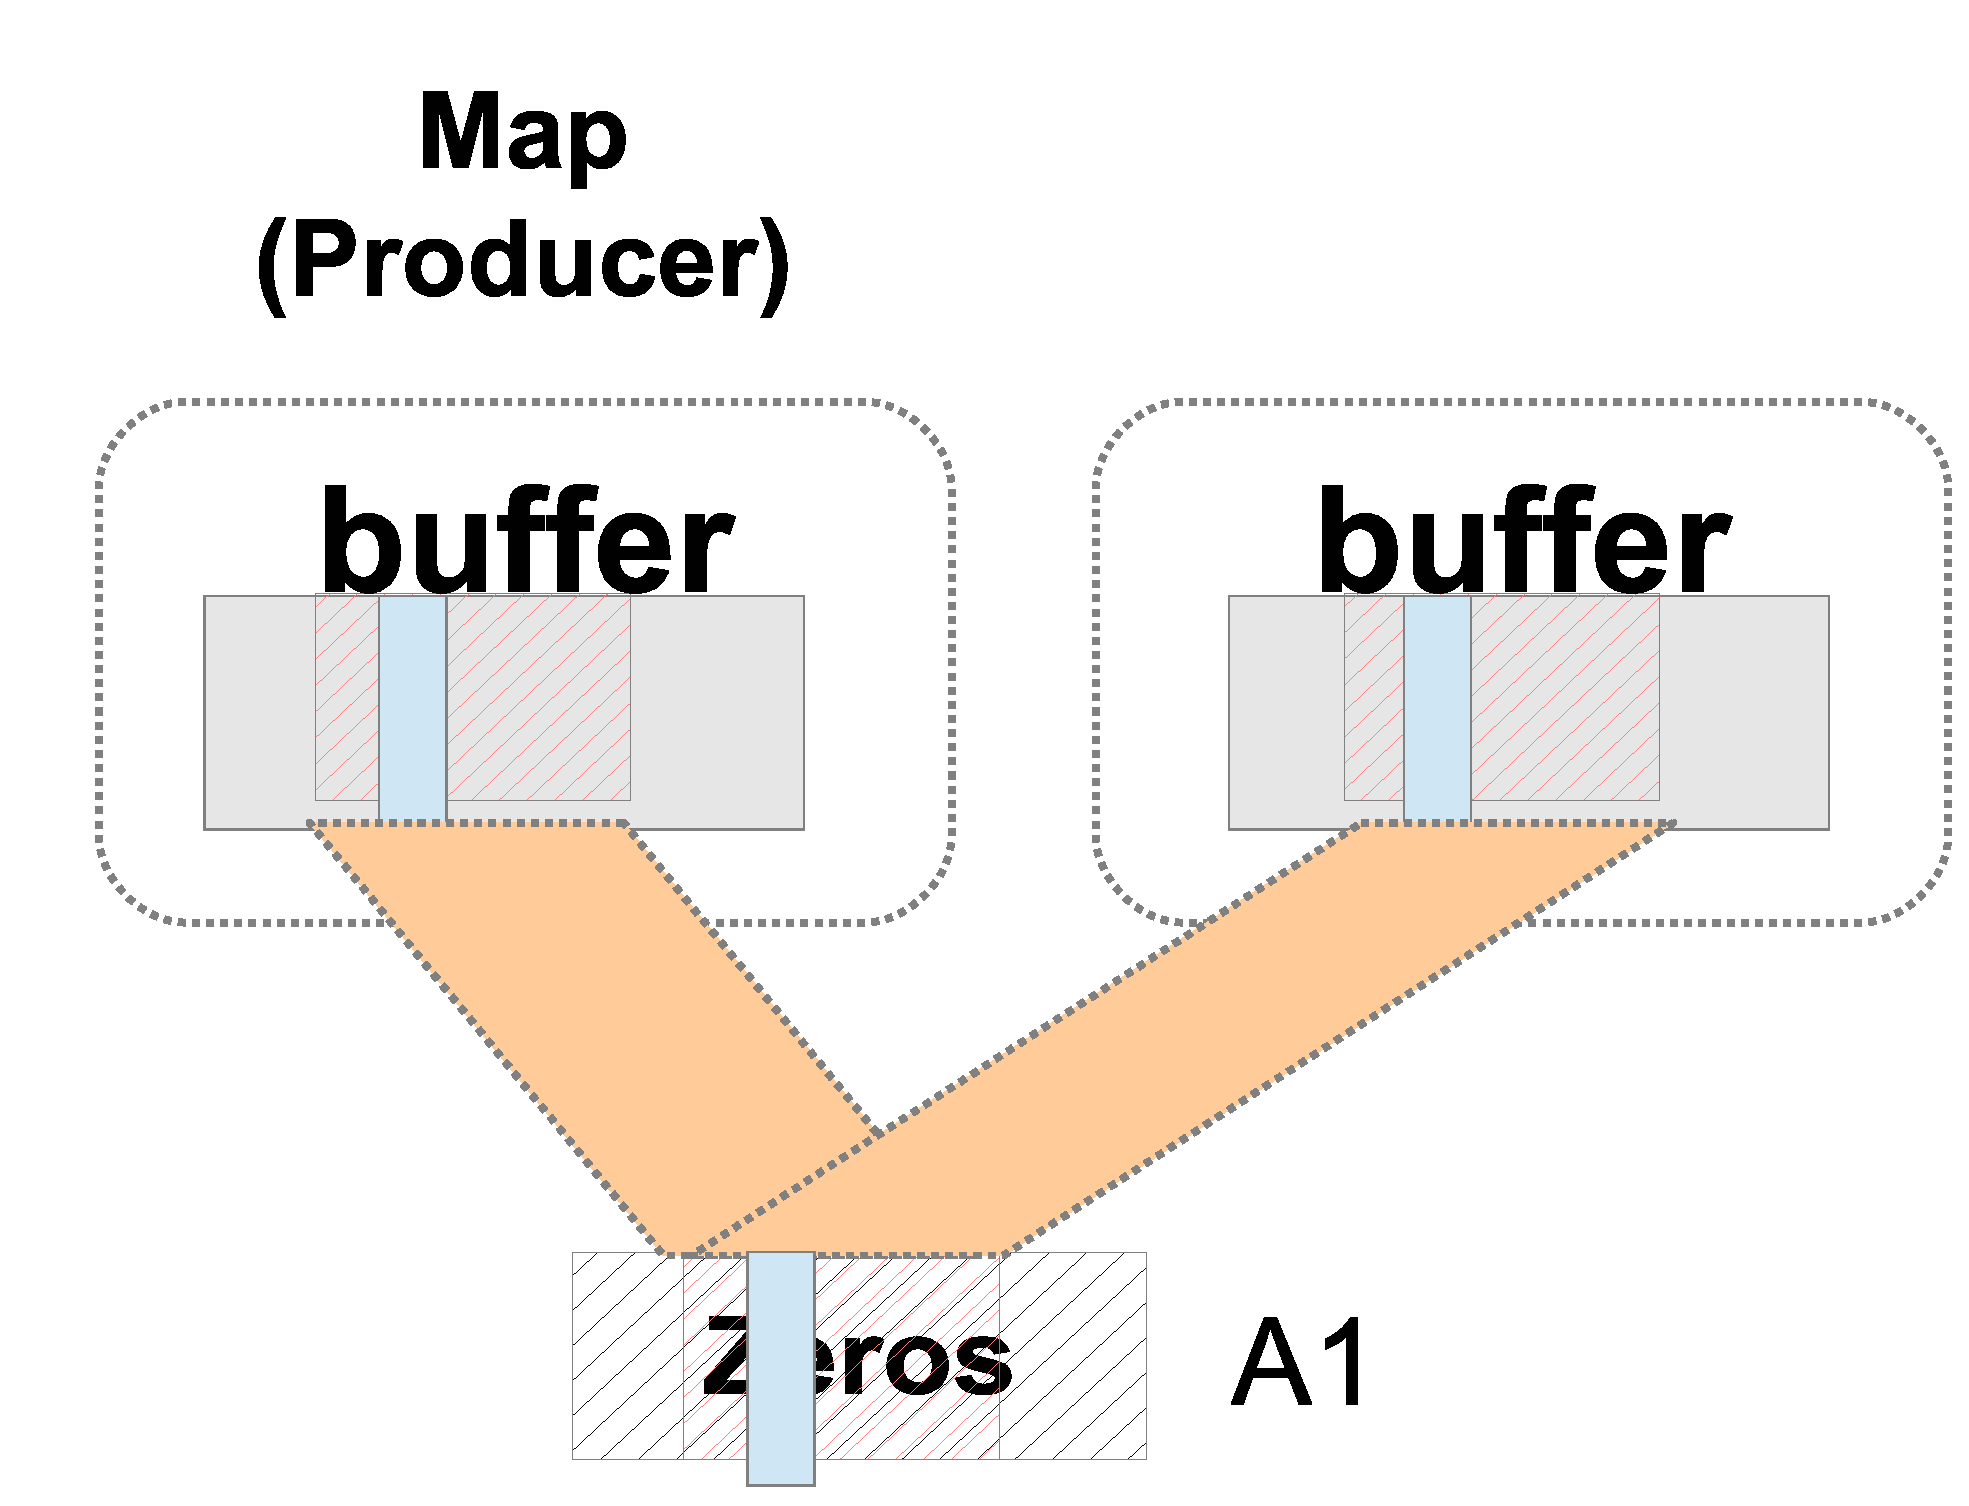
\includegraphics[width=0.23\textwidth]{eps/spmckern-ext0.eps}
% }
% \subfigure[]{
%  \label{fig:spmc:kernext:b}  
%  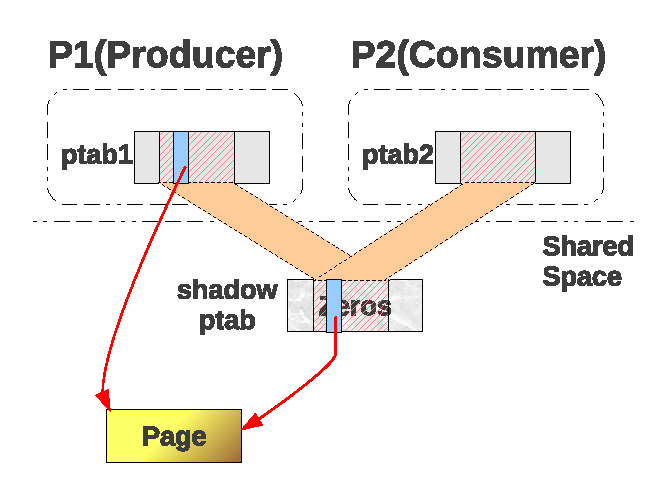
\includegraphics[width=0.23\textwidth]{eps/spmckern-ext2.eps}
% }
% \subfigure[]{
%  \label{fig:spmc:kernext:c}  
%  \includegraphics[width=0.23\textwidth]{eps/spmckern-ext3.eps}
% }
% \subfigure[]{
%  \label{fig:spmc:kernext:d}  
%  \includegraphics[width=0.23\textwidth]{eps/spmckern-ext4.eps}
% }
%\caption{Mechanism of SPMC virtual memory with lazy page mapping and space extension.}
%\label{fig:dmr:spmc}
%\end{figure*}

%最后,结合mapreduce来说明这种结构的优势在何处












